\documentclass[11pt,a4paper]{article}
\usepackage[utf8]{inputenc}
\usepackage[T1]{fontenc}
\usepackage[brazil]{babel}
\usepackage{lmodern}
\usepackage[margin=2.2cm]{geometry}
\usepackage{graphicx}
\usepackage{pdflscape}
\usepackage{tikz}
\usetikzlibrary{shapes.geometric,positioning,calc,fit}
\usepackage[normalem]{ulem}
\usepackage{booktabs}
\usepackage{tabularx}
\usepackage{longtable}
\usepackage{array}
\usepackage{enumitem}
\usepackage{float}
\usepackage{parskip}
\usepackage[hidelinks]{hyperref}

% =====================================================================
% Estilo dos diagramas ER/ERE -- notação Elmasri & Navathe,
% cores inspiradas na ferramenta TerraER
% (entidade verde, relacionamento amarelo, atributo lilás).
% Tamanhos de fonte podem ser redefinidos antes do \input.
% =====================================================================
\definecolor{terraEnt}{RGB}{186,242,186}
\definecolor{terraEntB}{RGB}{40,110,40}
\definecolor{terraRel}{RGB}{255,240,90}
\definecolor{terraRelB}{RGB}{120,100,0}
\definecolor{terraAtt}{RGB}{170,170,238}
\definecolor{terraAttB}{RGB}{40,40,120}

\providecommand{\erEntFont}{\scriptsize}
\providecommand{\erRelFont}{\tiny}
\providecommand{\erAttFont}{\tiny}
\providecommand{\erEntW}{2.3cm}
\providecommand{\erEntH}{0.7cm}
\providecommand{\erAttH}{0.42cm}

\tikzset{
  ent/.style={draw=terraEntB, semithick, rectangle, minimum width=\erEntW,
              minimum height=\erEntH, font=\sffamily\erEntFont, fill=terraEnt},
  went/.style={ent, double, double distance=1.5pt},
  rel/.style={draw=terraRelB, semithick, diamond, aspect=2.4, inner sep=1pt,
              font=\sffamily\erRelFont, fill=terraRel},
  irel/.style={rel, double, double distance=1.5pt},
  att/.style={draw=terraAttB, ellipse, inner sep=0.6pt, minimum height=\erAttH,
              font=\sffamily\erAttFont, fill=terraAtt},
  mval/.style={att, double, double distance=1pt},
  der/.style={att, dashed},
  spec/.style={draw, thick, circle, inner sep=0pt, minimum size=0.5cm,
               font=\sffamily\erEntFont, fill=white},
  tot/.style={double, double distance=1.6pt, line width=0.6pt},
  card/.style={midway, auto, inner sep=1.5pt, font=\sffamily\erEntFont},
  aggr/.style={draw=terraEntB, thick, rectangle, inner sep=0.35cm},
  sub/.style={midway, sloped, allow upside down, font=\small, inner sep=0pt},
}
\newcommand{\pk}[1]{\underline{#1}}
\newcommand{\ppk}[1]{\dashuline{#1}}


\newcolumntype{Y}{>{\raggedright\arraybackslash}X}
\newcolumntype{C}[1]{>{\centering\arraybackslash\hspace{0pt}}p{#1}}
\newcolumntype{L}[1]{>{\raggedright\arraybackslash\hspace{0pt}}p{#1}}

% Tabela de atributos de uma entidade
\newenvironment{atributos}{%
  \par\footnotesize
  \noindent\begin{tabular}{@{}L{3.0cm} L{4.9cm} C{1.6cm} C{1.6cm} C{1.9cm} C{1.3cm}@{}}
  \toprule
  Atributo & Semântica & Simples/\newline Composto &
  Mono/\newline Multival. & \mbox{Armazenado/}\newline Derivado & Chave\newline primária \\
  \midrule}{%
  \bottomrule
  \end{tabular}\par\medskip}

\newcommand{\entidade}[3]{%
  \subsubsection*{#1}
  Semântica: #2\par
  Atributos: #3\par\smallskip}

\begin{document}

% =====================================================================
% CAPA
% =====================================================================
\begin{titlepage}
  \centering
  {\large Universidade Federal de Ouro Preto -- UFOP\\
   Instituto de Ciências Exatas e Biológicas -- ICEB\\
   Departamento de Computação -- DECOM\par}
  \vspace{1.2cm}
  {\large BCC321 -- Banco de Dados I\\ Prof. Guilherme Tavares de Assis\par}
  \vspace{3cm}
  {\LARGE Trabalho Prático I\\[4pt] Modelagem Conceitual de Dados\par}
  \vspace{1cm}
  {\Large Sistema de Alocação de Quadras da UFOP\par}
  \vfill
  {\large
   Pedro Souza\\
   Luiz Felipe Bento\\
   Gabriel Canuto\\
   David Cristian\\
   Marcus Leandro\\
   Pedro Henrique Boseja\par}
  \vspace{2cm}
  {\large Ouro Preto -- 2026/2\par}
\end{titlepage}

\tableofcontents
\newpage

% =====================================================================
\section{Introdução e minimundo}
% =====================================================================


A UFOP possui diversos espaços esportivos -- quadras e campos de futebol --
distribuídos pelas unidades de Ouro Preto, Mariana e João Monlevade.
Esses espaços são disputados por alunos, atléticas e outras organizações para
lazer, treinos, campeonatos e aulas. Sem um controle centralizado surgem
conflitos de horário, reservas que não são utilizadas e falta de informação
sobre espaços em manutenção.

Este trabalho apresenta a modelagem conceitual de um sistema de banco de dados
para o agendamento dos espaços esportivos da UFOP. No sistema, alunos e
organizações realizam reservas em blocos de horário; funcionários
administram a agenda (abrem os horários de funcionamento dos espaços, bloqueiam espaços, cancelam
agendamentos e atendem chamados de suporte); e
administradores, desenvolvedores do sistema, gerenciam os funcionários.

O documento está organizado conforme o enunciado: a Seção~\ref{sec:req}
descreve os requisitos de dados; a Seção~\ref{sec:ere} apresenta o esquema
Entidade-Relacionamento Estendido (ERE); e a Seção~\ref{sec:dic} traz o
dicionário de dados.

% =====================================================================
\section{Requisitos de dados}\label{sec:req}
% =====================================================================

\subsection{Usuários e organizações}
\begin{enumerate}[label=R\arabic*., leftmargin=*, series=req]
  \item O sistema armazena os usuários. Cada usuário é identificado
        pelo seu CPF e possui nome (composto por primeiro nome e sobrenome),
        e-mail, um ou mais telefones e data de nascimento. A idade do usuário
        não é armazenada: ela é obtida a partir da data de nascimento.
  \item Todo usuário é, obrigatoriamente, de exatamente um dos três
        tipos a seguir (especialização disjunta e total):
        \begin{itemize}
          \item Usuário comum: aluno da UFOP que reserva espaços e
                participa de agendamentos. Matricula-se em um ou mais
                cursos (ver R3);
          \item Funcionário: servidor que administra a agenda dos
                espaços esportivos. Possui código de funcionário (valor
                único) e turno de trabalho;
          \item Administrador: desenvolvedor responsável pelo sistema.
                Possui nível de acesso.
        \end{itemize}
  \item Cada curso da UFOP possui código (único) e nome. Todo usuário comum
        está matriculado em pelo menos um curso, um aluno pode se matricular
        em vários cursos ao longo do tempo e um curso possui vários alunos
        (relacionamento M:N). Os dados da matrícula pertencem ao par
        aluno/curso e por isso ficam no relacionamento: número da matrícula
        (valor único), data de ingresso e situação (ativa ou inativa). Quando o
        aluno muda de curso, um novo par aluno/curso é registrado e o anterior
        passa a inativo, mas continua registrado, preservando o histórico.
  \item Um administrador gerencia vários funcionários, e todo funcionário é
        gerenciado por exatamente um administrador.
  \item O sistema armazena as organizações (atléticas, DCE, centros
        acadêmicos, departamentos). Cada organização possui código (único),
        nome e um ou mais telefones.
  \item Um agendamento é feito por um responsável, que pode ser um
        usuário comum ou uma organização (união). Nem todo usuário
        comum ou organização precisa ser responsável por algum agendamento.
\end{enumerate}

\subsection{Unidades (campus), espaços esportivos e modalidades}
\begin{enumerate}[resume*=req]
  \item Cada campus da UFOP possui código (único), nome e cidade.
  \item Cada espaço esportivo possui código (único), nome, capacidade
        máxima de pessoas e situação (disponível, em manutenção ou interditado).
        Todo espaço fica em exatamente um campus, e um campus pode possuir
        vários espaços.
  \item Todo espaço esportivo é de exatamente um dos tipos a seguir
        (especialização disjunta e total):
        \begin{itemize}
          \item Quadra: possui tipo de piso e indicação se é coberta;
          \item Campo: possui tipo de gramado.
        \end{itemize}
  \item Cada modalidade esportiva (futsal, futebol, vôlei, basquete etc.)
        possui código (único) e nome. Todo espaço suporta uma ou mais
        modalidades, e uma modalidade pode ser praticada em vários espaços.
        Cada par espaço--modalidade (por exemplo, ``futsal na quadra do
        ICEB'') é tratado como uma agregação, que pode ser reservada.
\end{enumerate}

\subsection{Horários e agendamentos}
\begin{enumerate}[resume*=req]
  \item Cada espaço possui horários de funcionamento: um funcionário abre o
        espaço em uma data, informando a hora de abertura e a hora de
        fechamento (por exemplo, dia 10/11, das 07:00 às 23:00). Um horário
        de funcionamento só existe vinculado ao seu espaço e é identificado pelo
        espaço juntamente com a data (entidade fraca). Cada horário de
        funcionamento é definido por um funcionário, e um funcionário pode
        definir vários.
  \item O período aberto de cada horário de funcionamento é dividido em
        blocos de horário de 1 hora, que são o tempo-limite de cada reserva.
        Por exemplo, se o espaço abre das 07:00 às 10:00, os blocos são
        07:00--08:00, 08:00--09:00 e 09:00--10:00. Cada bloco só existe
        dentro do seu horário de funcionamento e é identificado por ele
        juntamente com a hora de início (entidade fraca); possui também hora
        de fim, e a duração é calculada.
  \item Cada agendamento possui código (único) e status (pendente,
        confirmado, cancelado ou concluído). O número de participantes é
        calculado, e não armazenado. A data do agendamento é a data do
        horário de funcionamento dos blocos reservados.
  \item Todo agendamento é realizado por exatamente um responsável, ocupa um
        ou mais blocos de horário (por exemplo, dois blocos de 1 hora
        seguidos) e reserva exatamente um par espaço--modalidade (agregação).
        Cada bloco pode ser reservado por no máximo um agendamento. Um
        responsável e um par espaço--modalidade podem estar associados a
        vários agendamentos.
  \item Usuários comuns podem ser registrados como participantes de
        um agendamento. Um agendamento pode ter vários participantes, e um
        usuário comum pode participar de vários agendamentos.
  \item Um agendamento pode ser cancelado. O agendamento cancelado é uma
        subclasse de agendamento (especialização parcial, pois nem todo
        agendamento é cancelado) que registra a data do cancelamento e o
        motivo. Todo cancelamento é feito por exatamente um usuário -- o
        próprio aluno ou um funcionário.
\end{enumerate}

\subsection{Gestão e controle}
\begin{enumerate}[resume*=req]
  \item Um funcionário pode registrar bloqueios de espaços. Cada
        bloqueio possui código (único), período (composto por início e fim) e
        motivo (manutenção, evento, jogo oficial etc.), é registrado por
        exatamente um funcionário e se refere a exatamente um espaço.
  \item Qualquer usuário pode abrir chamados de suporte. Cada chamado
        possui número (único), descrição, data de abertura e status
        (aberto, em atendimento ou resolvido). Todo chamado é aberto por
        exatamente um usuário e pode ser atendido por um funcionário.
\end{enumerate}

% =====================================================================
\section{Esquema ERE}\label{sec:ere}
% =====================================================================

O esquema foi elaborado na notação adotada pelo livro-texto (Elmasri \&
Navathe), a mesma utilizada pela ferramenta TerraER:

\begin{itemize}[nosep]
  \item retângulo: entidade; retângulo duplo: entidade fraca;
  \item losango: relacionamento; losango duplo: relacionamento identificador;
  \item elipse: atributo; elipse dupla: multivalorado; elipse tracejada: derivado;
  \item atributo \pk{sublinhado}: chave; \ppk{sublinhado tracejado}: chave parcial;
  \item linha dupla: participação total; linha simples: participação parcial;
  \item círculo com d: especialização disjunta; círculo com
        U: união (categoria); o símbolo $\supset$ na linha indica a
        subclasse/categoria (sem círculo quando há uma única subclasse);
  \item retângulo envolvendo entidades e relacionamento: agregação.
\end{itemize}

O esquema atende aos requisitos mínimos do enunciado:
\begin{itemize}[nosep]
  \item 11 entidades (sem contar subclasses e categoria): USUARIO,
        CURSO, ORGANIZACAO, CAMPUS, ESPACO\_ESPORTIVO, MODALIDADE,
        HORARIO\_FUNCIONAMENTO, BLOCO\_HORARIO, AGENDAMENTO, BLOQUEIO e
        CHAMADO\_SUPORTE;
  \item 3 especializações: USUARIO $\rightarrow$ \{USUARIO\_COMUM,
        FUNCIONARIO, ADMINISTRADOR\} e ESPACO\_ESPORTIVO $\rightarrow$
        \{QUADRA, CAMPO\}, disjuntas e totais; AGENDAMENTO $\rightarrow$
        \{CANCELAMENTO\}, parcial;
  \item 1 união: RESPONSAVEL = USUARIO\_COMUM $\cup$ ORGANIZACAO, parcial;
  \item 1 agregação: [ESPACO\_ESPORTIVO -- SUPORTA -- MODALIDADE], que
        participa do relacionamento RESERVA com AGENDAMENTO.
\end{itemize}

O esquema completo é apresentado na Figura~\ref{fig:der} (página seguinte, em
paisagem). Para facilitar a leitura, as Figuras~\ref{fig:p1}
a~\ref{fig:p4} mostram o mesmo esquema dividido em partes.

\begin{landscape}
\begin{figure}[p]
  \centering
  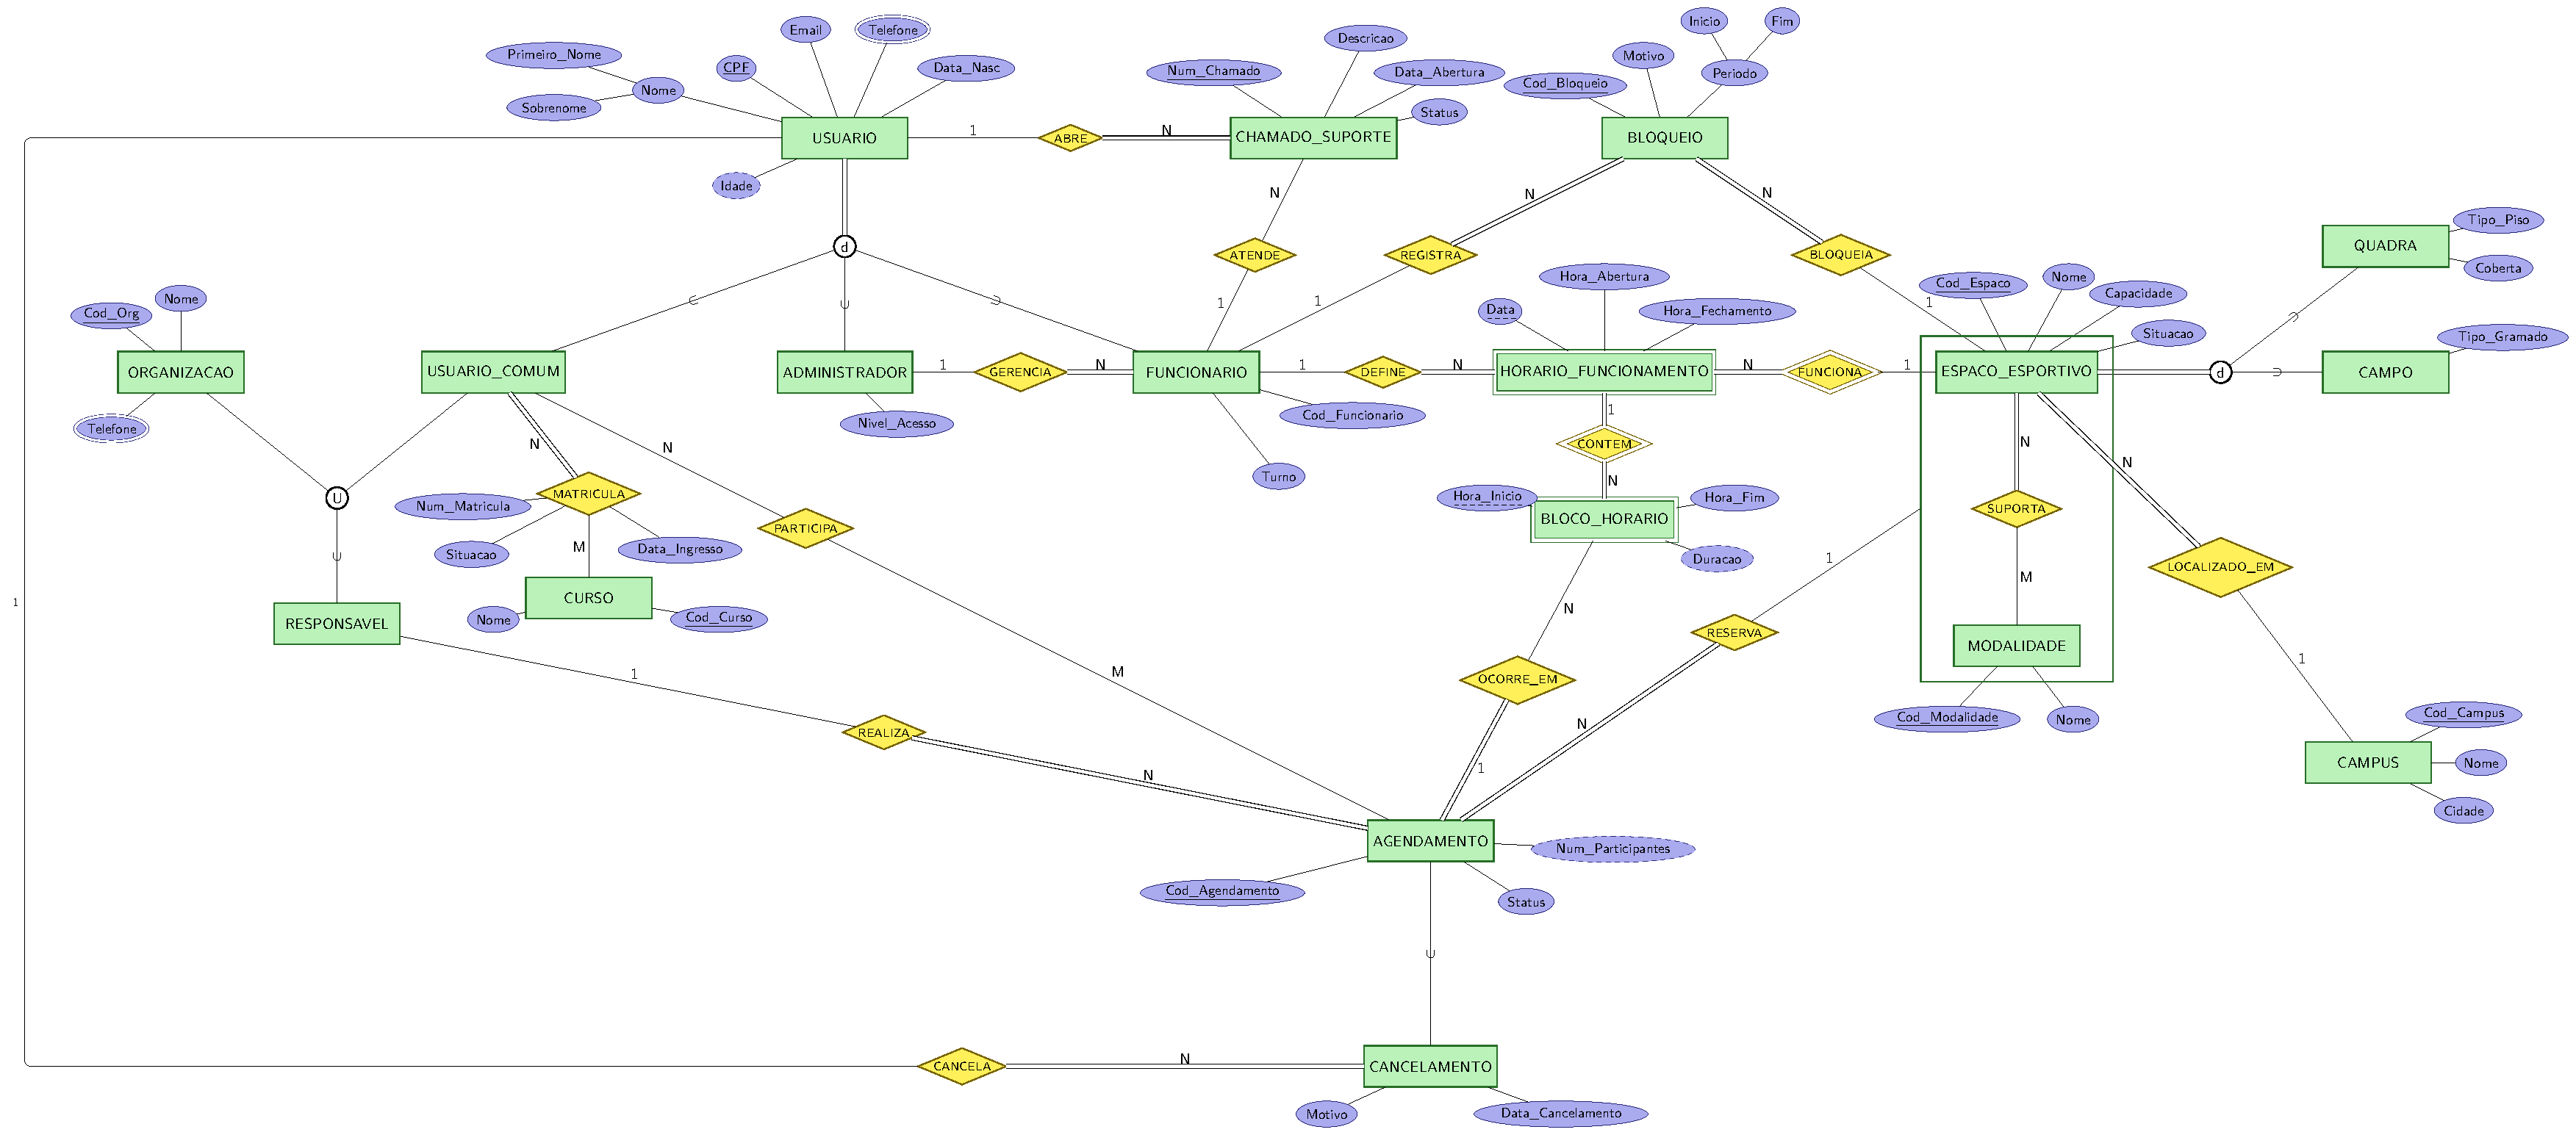
\includegraphics[width=\linewidth,height=0.9\textheight,keepaspectratio]{der.pdf}
  \caption{Esquema ERE completo do sistema.}
  \label{fig:der}
\end{figure}
\end{landscape}

\newcommand{\parte}[3]{%
  \begin{figure}[H]
    \centering
    \resizebox{\linewidth}{!}{\input{#1}}
    \caption{#2}\label{#3}
  \end{figure}}

\parte{parte1}{Detalhe: usuários, curso e matrícula, especialização de USUARIO e união RESPONSAVEL.}{fig:p1}
\parte{parte2}{Detalhe: espaços esportivos, especialização, campus, horário de funcionamento e agregação ESPACO--SUPORTA--MODALIDADE.}{fig:p2}
\parte{parte3}{Detalhe: agendamento, reserva da agregação, blocos de horário, participantes e cancelamento.}{fig:p3}
\parte{parte4}{Detalhe: gestão -- bloqueios, horários de funcionamento e suporte.}{fig:p4}

% =====================================================================
\section{Dicionário de dados}\label{sec:dic}
% =====================================================================

\subsection{Entidades e atributos}

Para cada entidade são apresentadas a semântica e a lista de atributos. Para
cada atributo são apresentadas a semântica e as categorias em que se enquadra.
Atributos componentes de um atributo composto aparecem recuados abaixo dele.
As subclasses herdam todos os atributos (inclusive a chave) da sua superclasse.

% ---------------------------------------------------------------------
\entidade{USUARIO}
  {representa toda pessoa cadastrada no sistema. É a superclasse da
   especialização disjunta e total em USUARIO\_COMUM, FUNCIONARIO e ADMINISTRADOR.}
  {CPF, Nome (Primeiro\_Nome, Sobrenome), Email, Telefone, Data\_Nasc, Idade.}
\begin{atributos}
  CPF & Número do CPF; identifica o usuário & Simples & Mono & Armazenado & Sim \\
  Nome & Nome completo do usuário & Composto & Mono & Armazenado & Não \\
  \quad Primeiro\_Nome & Primeiro nome & Simples & Mono & Armazenado & Não \\
  \quad Sobrenome & Sobrenome & Simples & Mono & Armazenado & Não \\
  Email & Endereço de e-mail & Simples & Mono & Armazenado & Não \\
  Telefone & Telefones de contato (um ou mais) & Simples & Multi & Armazenado & Não \\
  Data\_Nasc & Data de nascimento & Simples & Mono & Armazenado & Não \\
  Idade & Idade, calculada a partir de Data\_Nasc & Simples & Mono & Derivado & Não \\
\end{atributos}

\entidade{USUARIO\_COMUM (subclasse de USUARIO)}
  {aluno da UFOP que reserva espaços e participa de agendamentos.}
  {não possui atributos próprios além dos herdados de USUARIO; suas
   matrículas ficam no relacionamento MATRICULA com CURSO.}

\entidade{CURSO}
  {curso de graduação da UFOP em que os alunos se matriculam.}
  {Cod\_Curso, Nome.}
\begin{atributos}
  Cod\_Curso & Código que identifica o curso & Simples & Mono & Armazenado & Sim \\
  Nome & Nome do curso & Simples & Mono & Armazenado & Não \\
\end{atributos}

\entidade{FUNCIONARIO (subclasse de USUARIO)}
  {servidor da UFOP que administra a agenda dos espaços esportivos.}
  {Cod\_Funcionario, Turno (além dos herdados de USUARIO).}
\begin{atributos}
  Cod\_Funcionario & Código que identifica o funcionário no sistema (valor único) & Simples & Mono & Armazenado & Não \\
  Turno & Turno de trabalho (manhã, tarde ou noite) & Simples & Mono & Armazenado & Não \\
\end{atributos}

\entidade{ADMINISTRADOR (subclasse de USUARIO)}
  {desenvolvedor responsável pelo sistema; gerencia os funcionários.}
  {Nivel\_Acesso (além dos herdados de USUARIO).}
\begin{atributos}
  Nivel\_Acesso & Nível de permissão no sistema & Simples & Mono & Armazenado & Não \\
\end{atributos}

\entidade{ORGANIZACAO}
  {entidade estudantil ou institucional (atlética, DCE, centro acadêmico,
   departamento) que pode realizar agendamentos.}
  {Cod\_Org, Nome, Telefone.}
\begin{atributos}
  Cod\_Org & Código que identifica a organização & Simples & Mono & Armazenado & Sim \\
  Nome & Nome da organização & Simples & Mono & Armazenado & Não \\
  Telefone & Telefones de contato (um ou mais) & Simples & Multi & Armazenado & Não \\
\end{atributos}

\entidade{RESPONSAVEL (categoria / união)}
  {representa quem realiza um agendamento. É a união (parcial) de
   USUARIO\_COMUM e ORGANIZACAO: cada responsável é um usuário comum ou uma
   organização.}
  {não possui atributos próprios; cada instância herda os atributos da
   superclasse a que pertence.}

\entidade{CAMPUS}
  {unidade da UFOP onde ficam os espaços esportivos.}
  {Cod\_Campus, Nome, Cidade.}
\begin{atributos}
  Cod\_Campus & Código que identifica o campus & Simples & Mono & Armazenado & Sim \\
  Nome & Nome do campus & Simples & Mono & Armazenado & Não \\
  Cidade & Cidade onde se localiza o campus & Simples & Mono & Armazenado & Não \\
\end{atributos}

\entidade{ESPACO\_ESPORTIVO}
  {local físico da UFOP disponível para reserva. É a superclasse da
   especialização disjunta e total em QUADRA e CAMPO.}
  {Cod\_Espaco, Nome, Capacidade, Situacao.}
\begin{atributos}
  Cod\_Espaco & Código que identifica o espaço & Simples & Mono & Armazenado & Sim \\
  Nome & Nome do espaço & Simples & Mono & Armazenado & Não \\
  Capacidade & Número máximo de pessoas & Simples & Mono & Armazenado & Não \\
  Situacao & Disponível, em manutenção ou interditado & Simples & Mono & Armazenado & Não \\
\end{atributos}

\entidade{QUADRA (subclasse de ESPACO\_ESPORTIVO)}
  {quadra poliesportiva (futsal, vôlei, basquete etc.).}
  {Tipo\_Piso, Coberta (além dos herdados de ESPACO\_ESPORTIVO).}
\begin{atributos}
  Tipo\_Piso & Material do piso & Simples & Mono & Armazenado & Não \\
  Coberta & Indica se a quadra é coberta & Simples & Mono & Armazenado & Não \\
\end{atributos}

\entidade{CAMPO (subclasse de ESPACO\_ESPORTIVO)}
  {campo de futebol.}
  {Tipo\_Gramado (além dos herdados de ESPACO\_ESPORTIVO).}
\begin{atributos}
  Tipo\_Gramado & Gramado natural ou sintético & Simples & Mono & Armazenado & Não \\
\end{atributos}

\entidade{MODALIDADE}
  {esporte que pode ser praticado nos espaços esportivos.}
  {Cod\_Modalidade, Nome.}
\begin{atributos}
  Cod\_Modalidade & Código que identifica a modalidade & Simples & Mono & Armazenado & Sim \\
  Nome & Nome da modalidade & Simples & Mono & Armazenado & Não \\
\end{atributos}

\entidade{HORARIO\_FUNCIONAMENTO (entidade fraca)}
  {período em que um espaço fica aberto para agendamentos em uma data
   (por exemplo, das 07:00 às 23:00). É identificado pelo espaço esportivo
   (relacionamento identificador FUNCIONA) juntamente com a chave parcial Data.}
  {Data, Hora\_Abertura, Hora\_Fechamento.}
\begin{atributos}
  Data & Data em que o espaço abre & Simples & Mono & Armazenado & Parcial \\
  Hora\_Abertura & Hora de abertura do espaço & Simples & Mono & Armazenado & Não \\
  Hora\_Fechamento & Hora de fechamento do espaço & Simples & Mono & Armazenado & Não \\
\end{atributos}

\entidade{BLOCO\_HORARIO (entidade fraca)}
  {bloco de 1 hora em que o período de um horário de funcionamento é
   dividido (por exemplo, 07:00--08:00); é a unidade reservada pelos
   agendamentos. É identificado pelo horário de funcionamento
   (relacionamento identificador CONTEM) juntamente com a chave parcial
   Hora\_Inicio.}
  {Hora\_Inicio, Hora\_Fim, Duracao.}
\begin{atributos}
  Hora\_Inicio & Hora de início do bloco & Simples & Mono & Armazenado & Parcial \\
  Hora\_Fim & Hora de término do bloco & Simples & Mono & Armazenado & Não \\
  Duracao & Hora\_Fim $-$ Hora\_Inicio & Simples & Mono & Derivado & Não \\
\end{atributos}

\entidade{AGENDAMENTO}
  {reserva de um par espaço--modalidade, feita por um responsável, em um ou mais
   blocos de horário. É a superclasse da especialização
   parcial em CANCELAMENTO.}
  {Cod\_Agendamento, Status, Num\_Participantes.}
\begin{atributos}
  Cod\_Agendamento & Código que identifica o agendamento & Simples & Mono & Armazenado & Sim \\
  Status & Pendente, confirmado, cancelado ou concluído & Simples & Mono & Armazenado & Não \\
  Num\_Participantes & Quantidade de participantes (contagem em PARTICIPA) & Simples & Mono & Derivado & Não \\
\end{atributos}

\entidade{CANCELAMENTO (subclasse de AGENDAMENTO)}
  {agendamento que foi cancelado. Especialização parcial: só os agendamentos
   cancelados pertencem a esta subclasse.}
  {Data\_Cancelamento, Motivo (além dos herdados de AGENDAMENTO).}
\begin{atributos}
  Data\_Cancelamento & Data em que o agendamento foi cancelado & Simples & Mono & Armazenado & Não \\
  Motivo & Justificativa do cancelamento & Simples & Mono & Armazenado & Não \\
\end{atributos}

\entidade{BLOQUEIO}
  {período em que um espaço esportivo fica indisponível para reservas.}
  {Cod\_Bloqueio, Periodo (Inicio, Fim), Motivo.}
\begin{atributos}
  Cod\_Bloqueio & Código que identifica o bloqueio & Simples & Mono & Armazenado & Sim \\
  Periodo & Intervalo do bloqueio & Composto & Mono & Armazenado & Não \\
  \quad Inicio & Data/hora de início & Simples & Mono & Armazenado & Não \\
  \quad Fim & Data/hora de fim & Simples & Mono & Armazenado & Não \\
  Motivo & Manutenção, evento, jogo oficial etc. & Simples & Mono & Armazenado & Não \\
\end{atributos}

\entidade{CHAMADO\_SUPORTE}
  {solicitação de ajuda aberta por um usuário e atendida por um funcionário.}
  {Num\_Chamado, Descricao, Data\_Abertura, Status.}
\begin{atributos}
  Num\_Chamado & Número que identifica o chamado & Simples & Mono & Armazenado & Sim \\
  Descricao & Descrição detalhada & Simples & Mono & Armazenado & Não \\
  Data\_Abertura & Data de abertura & Simples & Mono & Armazenado & Não \\
  Status & Aberto, em atendimento ou resolvido & Simples & Mono & Armazenado & Não \\
\end{atributos}

% ---------------------------------------------------------------------
\subsection{Relacionamentos}

Para cada relacionamento são apresentadas as entidades envolvidas, a razão de
cardinalidade e a restrição de participação de cada entidade.

{\small
\begin{longtable}{@{}L{3.2cm} L{5.4cm} C{1.3cm} L{5.3cm}@{}}
  \toprule
  Relacionamento & Entidades envolvidas & Card. & Participação e semântica \\
  \midrule
  \endhead
  \bottomrule
  \endfoot
  REALIZA & RESPONSAVEL -- AGENDAMENTO & 1:N & Responsável parcial; Agendamento total. Indica quem fez a reserva. \\
  SUPORTA & ESPACO\_ESPORTIVO -- MODALIDADE & N:M & Espaço total; Modalidade parcial. Modalidades possíveis em cada espaço. Forma a agregação reservada pelos agendamentos. \\
  RESERVA & AGENDAMENTO -- agregação [ESPACO\_ESPORTIVO -- SUPORTA -- MODALIDADE] & N:1 & Agendamento total; agregação parcial. Par espaço--modalidade reservado. \\
  OCORRE\_EM & AGENDAMENTO -- BLOCO\_HORARIO & 1:N & Agendamento total (ocupa ao menos um bloco); Bloco parcial (pode estar livre). Cada bloco é reservado por no máximo um agendamento. \\
  CONTEM (identificador) & HORARIO\_FUNCIONAMENTO -- BLOCO\_HORARIO & 1:N & Ambas totais: todo horário de funcionamento é dividido em blocos, e todo bloco pertence a um horário de funcionamento (entidade fraca). \\
  MATRICULA & USUARIO\_COMUM -- CURSO & N:M & Usuário comum total (todo aluno tem ao menos uma matrícula); Curso parcial. Possui atributos próprios (ver Seção~\ref{sec:atrrel}). Guarda o histórico de cursos do aluno. \\
  PARTICIPA & USUARIO\_COMUM -- AGENDAMENTO & N:M & Ambas parciais. Alunos que participam do agendamento. \\
  CANCELA & USUARIO -- CANCELAMENTO & 1:N & Usuário parcial; Cancelamento total. Usuário que efetuou o cancelamento. \\
  FUNCIONA (identificador) & ESPACO\_ESPORTIVO -- HORARIO\_FUNCIONAMENTO & 1:N & Espaço parcial; Horário de funcionamento total (entidade fraca). \\
  DEFINE & FUNCIONARIO -- HORARIO\_FUNCIONAMENTO & 1:N & Funcionário parcial; Horário de funcionamento total. Funcionário que abriu o espaço. \\
  LOCALIZADO\_EM & ESPACO\_ESPORTIVO -- CAMPUS & N:1 & Espaço total; Campus parcial. \\
  REGISTRA & FUNCIONARIO -- BLOQUEIO & 1:N & Funcionário parcial; Bloqueio total. \\
  BLOQUEIA & BLOQUEIO -- ESPACO\_ESPORTIVO & N:1 & Bloqueio total; Espaço parcial. \\
  ABRE & USUARIO -- CHAMADO\_SUPORTE & 1:N & Usuário parcial; Chamado total. \\
  ATENDE & FUNCIONARIO -- CHAMADO\_SUPORTE & 1:N & Ambas parciais (o chamado pode ainda não ter sido atendido). \\
  GERENCIA & ADMINISTRADOR -- FUNCIONARIO & 1:N & Administrador parcial; Funcionário total. \\
\end{longtable}}

% ---------------------------------------------------------------------
\subsection{Atributos de relacionamentos}\label{sec:atrrel}

\entidade{MATRICULA (relacionamento USUARIO\_COMUM -- CURSO)}
  {matrícula de um aluno em um curso. Os atributos dependem do par
   aluno/curso, por isso pertencem ao relacionamento e não às entidades.}
  {Num\_Matricula, Data\_Ingresso, Situacao.}
\begin{atributos}
  Num\_Matricula & Número da matrícula do aluno no curso (valor único) & Simples & Mono & Armazenado & Não \\
  Data\_Ingresso & Data de ingresso do aluno no curso & Simples & Mono & Armazenado & Não \\
  Situacao & Ativa ou inativa (curso anterior, após mudança) & Simples & Mono & Armazenado & Não \\
\end{atributos}

% ---------------------------------------------------------------------
\subsection{Especializações, união e agregação}

{\small
\begin{tabularx}{\linewidth}{@{}L{2.8cm} L{6.6cm} Y@{}}
  \toprule
  Construção & Envolvidos & Restrições \\
  \midrule
  Especialização & USUARIO $\rightarrow$ USUARIO\_COMUM, FUNCIONARIO, ADMINISTRADOR &
    Disjunta (d) e total: todo usuário é de exatamente um tipo. \\
  Especialização & ESPACO\_ESPORTIVO $\rightarrow$ QUADRA, CAMPO &
    Disjunta (d) e total: todo espaço é de exatamente um tipo. \\
  Especialização & AGENDAMENTO $\rightarrow$ CANCELAMENTO &
    Parcial: nem todo agendamento é cancelado. \\
  União (categoria) & RESPONSAVEL = USUARIO\_COMUM $\cup$ ORGANIZACAO &
    Parcial: nem todo usuário comum ou organização é responsável. \\
  Agregação & [ESPACO\_ESPORTIVO -- SUPORTA -- MODALIDADE] &
    Tratada como entidade de nível mais alto; participa de RESERVA com AGENDAMENTO. \\
  \bottomrule
\end{tabularx}}

\end{document}
